\section*{Création de notre data warehouse}
\addcontentsline{toc}{chapter}{Création de notre data warehouse}

\subsection*{Choix et récupération des données}

\addcontentsline{toc}{section}{Choix et récupération des données}

Afin de répondre à la problématique de départ, nous avons décidé de nous intéresser uniquement aux protéines humaines ayant été publiées, et plus particulièrement à celles disponibles sur la base de données \emph{uniprot}.

En effet, la requête [\emph{(homo sapiens) AND reviewed:yes}] sur cette base de données permet d'obtenir 26 070 protéines, ce qui est suffisant pour obtenir des résultats exploitables sans que cela ne devienne trop chronophage en terme de temps de traitement et d'analyse.

Nous récupérons donc les données sous la forme d'un fichier XML nous permettant de lire et de traiter facilement les données (parse de fichier texte). Les balises propres au système xml (<balise> information <$/$balise>) facilitant la récupération des données d'inter\^et.

\subsection*{Préparation des données}

\addcontentsline{toc}{section}{Préparation des données}
La préparation des données est indispensable car les données récupérées peuvent être incomplètes, bruitées ou incohérentes.\\
Nous avons remarqué que certaines protéines n'étaient pas des protéines humaines mais appartenaient à des virus, nous les avons donc supprimées. De plus, certaines protéines n'avaient pas de structure secondaire, nous avons décidé de ne pas les prendre en compte pour la création de notre data warehouse.\\
%\subsubsection*{Nettoyage}
%\addcontentsline{toc}{subsection}{Nettoyage}
Pour préparer les données, nous avons sélectionné les balises correspondant aux critères que nous prendrons en compte dans notre analyse :
\renewcommand\labelitemi{\textbullet}
\begin{itemize}
\item accession number (id)
\item name/full name
\item tissue
\item sequence length
\item feature type ="strand  - helix - turn"\\
\end{itemize}

Cette récupération se fait grâce à un programme python que nous avons écrit, nous permettant de "parser" le fichier XML précédemment acquis. Ainsi seules les données d'intérêt sont récupérées.\\

Ce script comporte deux parties, nous supprimons d'abord les balises qui ne sont pas utiles pour notre étude.
Nous ajoutons ensuite des données calculées au fichier précédent qui vont nous permettre de créer les clusters par la suite. Il s'agit de:
\begin{itemize}
\item Le nombre et le pourcentage d'hélices, de feuillets et de coudes dans la protéine.
\item Le pourcentage d'hydrophobicité.
\item Le pHi (point isoélectrique) qui a été déterminé à l'aide de la fonction\\ \texttt{isoelectric\_point()} présente dans BioPython.
\item Le nombre de cystéines.
\end{itemize}

Nous avons également supprimé les informations dupliquées (identifiants, noms etc).
Nous obtenons ainsi un fichier XML contenant uniquement les données que nous avons sélectionnées. Il contient 4441 protéines.

A partir de ce fichier et pour faciliter la création des clusters, nous avons décidé de créer trois tables.(cf figure table)
\begin{description}
\item[La table protéine] comprend toutes les données relatives à la protéine tel que le numéro d'accession, son nom complet, sa longueur et une liste contenant ses localisations.
\item[La table Structure] contient toutes les informations de structure de la protéine: le nombre et le pourcentage d'hélices, de feuillets et de coudes ainsi que le nombre de cystéines qu'elle possède.
\item[La table des propriétés chimiques] contient le pourcentage d'hydrophobicité et le pHi de la protéine.
\end{description}
Ses tables sont en fait des dictionnaires dans lesquels la clé est le numéro d'accession de la protéine. La valeur associée à la clé est un autre dictionnaire dans lequel les clés sont les noms des paramètres.

\begin{figure}
\begin{center}
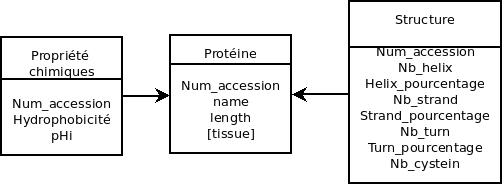
\includegraphics[scale=0.5]{figtable.png}
\caption{Schéma des tables du Data Warehouse}
\end{center}
\end{figure}

\section*{Critères choisis}
\addcontentsline{toc}{section}{Critères choisis}
Nous avons choisi 6 critères.

\subsection*{Taille de la chaîne}
\addcontentsline{toc}{subsection}{Taille de la cha\^ine}
Les protéines sont constituées d'une succession d'acides aminés reliés entre eux par des liaisons peptidiques. La taille d'une protéine est ainsi définie par le nombre d'acides aminés qu'elle contient. Cette taille étant très variable, les protéines ayant des tailles très différentes n'auront pas les m\^emes propriétés, ce critère constitue donc un bon premier niveau de clusterisation.

\subsection*{Structure tridimensionnelle}
\addcontentsline{toc}{subsection}{Structure tridimensionnelle}
Une protéine peut être décrite par un enchaînement de structures secondaires (hélices alpha, feuillets beta et coude) qui ont une influence sur son repliement.\\

\subsection*{Hydrophobicité}
\addcontentsline{toc}{subsection}{Hydrophobicité}
L'hydrophobicité d'une protéine est déterminée à partir du nombre d'acides aminés hydrophobes qu'elle possède.
Nous avons calculé un index d'hydrophobicité (GRAVY: Grand average of hydropathicity index,Kyte and Doolittle) qui indique la solubilité d'une protéine. Si la valeur est positive, la protéine est hydrophobe, sinon elle est hydrophile.
Son caractère hydrophobe ou hydrophile influence :
\begin{itemize}
\item Sa localisation au niveau cellulaire (cytoplasme ou membrane)
\item Son repliement (acides aminés hydrophobes à l'intérieur ou l'extérieur de la protéine selon sa localisation cellulaire) 
\end{itemize}


\subsection*{Nombre de cystéines}
\addcontentsline{toc}{subsection}{Nombre de cystéines}
Les ponts disulfures se forment au sein d'une protéine entre deux cystéines et créent des liaisons inter-chaines. Ils ont donc une influence sur la structure tridimensionnelle de la protéine.\\
%La formation des clusters de cystéine suit le m\^eme procédé que celui de la structure tridimensionnelle. Nous arr\^etons la formation lorsque chaque cluster d'hydrophobcité a été divisé en quatre.

\subsection*{pHi}
\addcontentsline{toc}{subsection}{pHi}
Le pHi est le pH isoéléctrique d'une protéine, c'est à dire le pH auquel cette protéine a une charge nulle et donc limite son déplacement dans un champ électrique physiologique.
Au dessus de ce pH, la protéine est chargée négativement (pH basique) et inversement, en dessous elle est chargée positivement (pH acide).\\
Lorsqu'une protéine est dans un milieu égal à son pHi cela met en évidence différentes propriétés, telles que:
\begin{itemize}
\item Sa solubilité qui est minimale,
\item Sa mobilité électrophorétique qui lui permet de migrer plus vers un milieu qu'un autre,
\item Son isoélectrofocalisation (IEF) qui repose sur ses peptides amphotères qui vont charger la protéine négativement ou positivement selon le milieu.
\end{itemize}
%La formation des clusters de pHi suit le m\^eme procédé que celui des précédentes formations. Nous arr\^etons la formation lorsque chaque cluster de cystéines a été divisé en quatre.

\subsection*{Localisation}
\addcontentsline{toc}{subsection}{Localisation}
Les protéines sont des constituants de nos organes et participent à la composition de la matrice de chacun de nos organes, tissus ainsi que nos cellules.\\
Une protéine a des fonctions déterminées qui peuvent être utiles dans différents organes, voisins ou non. 





